
\section{DP for TSP}
\begin{frame}{}
  \begin{center}
    {\bf Part II -- DP for Travelling Salesman Problems}
  \end{center}
\end{frame}

\begin{frame}[fragile]
  \frametitle{TSP Problem -- Blackbeard the Pirate}

  {\smaller

    \begin{block}{}
      Blackbeard has to \structure{collect all treasures} (up to 10)
      in the island. He \alert{cannot cross} water or trees, and he
      must stay 1 square away from natives.

      \medskip

      Black beard speed is 1 square / second. How long does it take
      to get all treasure and return to the ship?
    \end{block}

\begin{verbatim}
10 10
~~~~~~~~~~       ~ -- Water, can't cross
~~!!!###~~       # -- Trees, can't cross
~##...###~       ! -- Treasure, get these!
~#....*##~       . -- Just sand
~#!..**~~~       * -- Natives, don't get close here.
~~....~~~~       @ -- Landing point, start and return here.
~~~....~~~
~~..~..@~~       The solution for this case is: 32
~#!.~~~~~~       QUIZ: How to solve this problem?
~~~~~~~~~~
0 0
\end{verbatim}
}
\end{frame}

\subsection{Problem Solution -- Decomposition}
\begin{frame}[fragile]
  \frametitle{Blackbeard the Pirate -- Problem Idea}

    \begin{block}{One way to solve this problem is to break it into two parts:}
      \begin{enumerate}
      \item Create a treasure path graph from the input map
      \item Small number of treasures: Find TSP of treasure path
      \end{enumerate}
    \end{block}

    {\smaller
\begin{verbatim}
10 10
~~~~~~~~~~       ~ -- Water, can't cross
~~!!!###~~       # -- Trees, can't cross
~##...###~       ! -- Treasure, get these!
~#....*##~       . -- Just sand
~#!..**~~~       @ -- Landing point, return here.
~~....~~~~
~~~....~~~
~~..~..@~~
~#!.~~~~~~
~~~~~~~~~~
0 0
\end{verbatim}
  }
\end{frame}

\begin{frame}[fragile]
  \frametitle{Blackbeard -- Extracting the graph}

  {\smaller
\begin{verbatim}
10 10
~~~~~~~~~~  ##########  # -- Obstacle (waters and trees)
~~!!!###~~  ##345#####  X -- Obstacles (natives, just for clarity)
~##...###~  ###..X####  . -- Path
~#....*##~  ##..XXX###  0-9 -- Nodes
~#!..**~~~  ##2.XXX###
~~....~~~~  ##..XX####
~~~....~~~  ###....###
~~..~..@~~  ##..#..0##
~#!.~~~~~~  ##1.######
~~~~~~~~~~  ##########
0 0
\end{verbatim}

\begin{itemize}
\item We can simply the graph into obstacles, paths and goals
\item We are only interested in the treasures and goals, so how to find the
  pairwise distance between treasures?
\item \alert{Answer}: \only<2>{BFS from each treasure/start point}
\item The result is a small graph with {\bf at most} 11 vertices.
\end{itemize}

  }
\end{frame}

\begin{frame}[fragile]
  \frametitle{Blackbeard -- Extracting the graph}
  \begin{columns}
    \column{0.5\textwidth}

  {\smaller
\begin{verbatim}
##########
##345#####
###..X####
##..XXX###     BFS from each vertex
##2.XXX###     ------------------->
##..XX####     Not all paths shown
###....###
##..#..0##
##1.######
##########
\end{verbatim}}

    \column{0.5\textwidth}
  \begin{center}
    \begin{tikzpicture}[transform shape,label/.style={thin, draw=black, align=center,fill=white,font=\smaller},scale=1.1]
      \node[red vertex] (S) at (3,0) {0};
      \node[vertex] (ta) at (0,0) {1};
      \node[vertex] (tb) at (0,1.5) {2};
      \node[vertex] (tc) at (0,3) {3};
      \node[vertex] (td) at (1,3) {4};
      \node[vertex] (te) at (2,3) {5};
      \draw[edge] (S) -- node[label] {$8$} (ta);
      \draw[edge] (S) -- node[label] {$8$} (tb);
      \draw[edge] (S) -- node[label] {$10$} (td);
      \draw[edge] (td) -- node[label] {$1$} (tc);
      \draw[edge] (td) -- node[label] {$1$} (te);
      \draw[edge] (td) -- node[label] {$4$} (tb);
      \draw[edge] (tb) -- node[label] {$6$} (ta);
      \draw[edge] (S) -- node[label] {$11$} (te);
      \draw[edge] (tb) -- node[label] {$5$} (tc);
    \end{tikzpicture}
  \end{center}
  \end{columns}

  \begin{center}
    How do we find the minimal cycle starting in {\bf S}, passing by all vertices?
  \end{center}
\end{frame}

%% Explain TSP with DP and bit (Page 110)

\subsection{Traveling Salesman Problems}

\begin{frame}
  \frametitle{The Traveling Salesman Problem (TSP)}

  {\smaller
    \begin{block}{Problem Definition}
      You have $n$ cities, and their distances. Calculate the cost of
      the \structure{tour} that starts and ends at a city $s$, passing
      through all other cities.

      \medskip

      Exactly what we need! The path for all treasure!
  \end{block}
  \begin{center}
    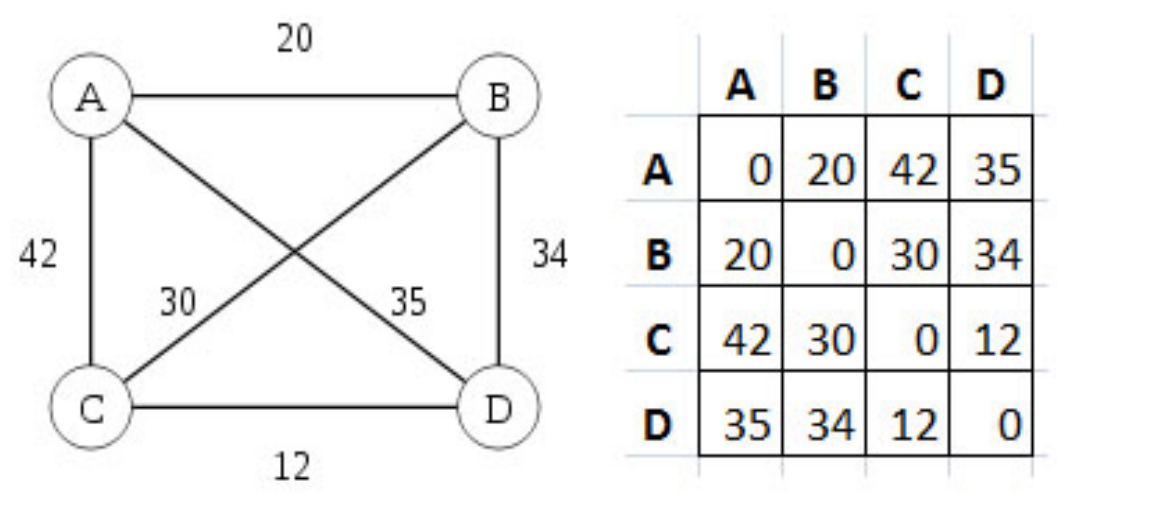
\includegraphics[width=0.5\textwidth]{../img/tsp_example}
  \end{center}

  In the graph above, we have $n=4$ cities and the minimal tour is
  A-B-C-D-A, with cost $20+30+12+35=97$.

  \medskip

  \alert{QUIZ:} What is the cost of solving TSP with complete search?
  }

  \hrulefill

  \hfill{\tiny Image from Steven Halim -- ``Competitive Programming''}

\end{frame}

\begin{frame}
  \frametitle{Characteristics of TSP}

  {\smaller
    \begin{block}{}
      \begin{itemize}
      \item A complete search for TSP costs $O(n!*n)$ -- \alert{Search
        each city permutation}.
      \item TSP is a {\bf NP-hard} problem. This means that there is
        no known polinomial algorithm to solve it.
      \item \alert{However!} For small values of $n$, there are some
        hacks to make the solution faster.
      \end{itemize}
    \end{block}

    \begin{exampleblock}{DP approach to TSP}
      The complete search for the TSP contains many \alert{repeated subsolutions}:
      \begin{itemize}
      \item S--A--B--C--$\ldots$--S
      \item S--B--A--C--$\ldots$--S
      \end{itemize}
      The minimum cost for C--$\ldots$--S is the same. Can we use
      \emph{memoization} to remember this cost?
    \end{exampleblock}
  }
\end{frame}

\begin{frame}
  \frametitle{DP approach to TSP (1) -- Idea}
    \begin{block}{}
      \begin{itemize}
      \item We have already visited the cities $S = \{s_1,s_2,\ldots,s_n\}, s_i \neq 0$
      \item We are {\bf now} in city $s_k \in S$
      \item What is the shortest path from $s_k$ to $0$, that passes in all cities $s_j \notin S$ ?
      \end{itemize}

      DP induction: shortest\_path($S$,$s_k$)
    \end{block}
    \begin{center}
      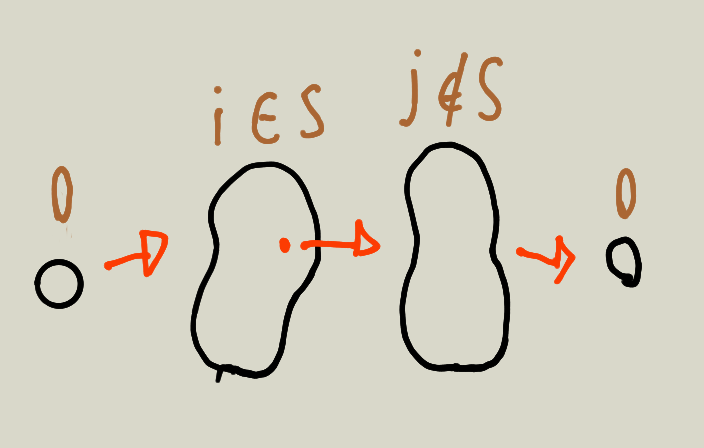
\includegraphics[width=0.4\textwidth]{img/DP_TSP}
    \end{center}
\end{frame}

\begin{frame}
  \frametitle{DP approach to TSP (2) -- DP Recurrence}

  {\smaller
    \begin{center}
      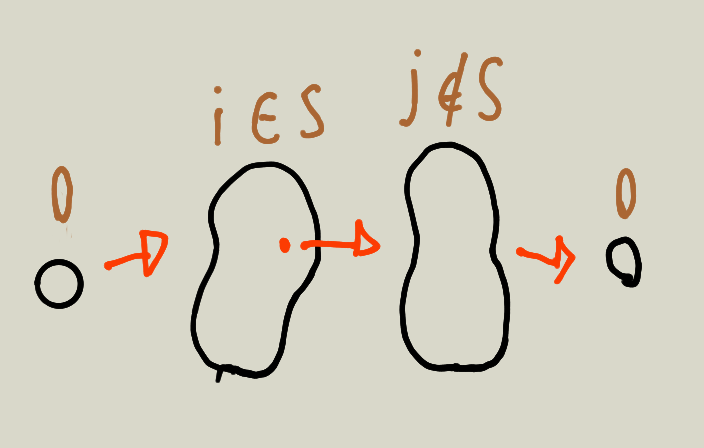
\includegraphics[width=0.35\textwidth]{img/DP_TSP}
    \end{center}
    \begin{block}{}
      \begin{itemize}
      \item We have visited all cities, and must return to the origin:\\
        shortest\_path($S_{\text{all}},s_k$) = $D(s_k,0)$
      \item We have visited some cites ($S$), and must find the next one:\\
        shortest\_path($S,s_k$) = $\text{min}_{s_i\notin S}
        (D(s_k,s_i) + \text{shortest\_path}(S\cup s_i,s_i))$
      \item Initial call:\\
        shortest\_path($S = \emptyset$,0)
      \end{itemize}
    \end{block}
  }
\end{frame}

\begin{frame}
  \frametitle{DP approach to TSP (3) -- Implementation}

    \begin{exampleblock}{}
      \begin{itemize}
      \item Our DP table is (\emph{all sets},\emph{all cities}) -- $2^n * n$
      \item We can represent a set of cities using a \structure{bitmask}
      \item At each call, we loop through all cities, so the complexity is $(O(2^n*n^2))$

        \bigskip

      \item TSP using full search: $O(n!*n)$
      \item TSP using DP: $O(2^n*n^2)$ -- Still low, but much better!
      \end{itemize}
    \end{exampleblock}
\end{frame}

\begin{frame}[fragile]
  \frametitle{DP approach to TSP (4) -- Sample Code}

{\smaller
  \begin{exampleblock}{}
\begin{verbatim}
int dp[n][1<<n] = -1
start = 0

visit(p,v):
   if (v == (1<<n) - 1):
      return cost[p][start]
   if dp[p][v] != -1
      return dp[p][v]

   tmp = MAXINT
   for i in n:
       if not(v && (1 << i):
           tmp = min(tmp,
                     cost[p][i] + visit(i, v | (1<<i)))

   dp[p][v] = tmp
   return tmp
\end{verbatim}
  \end{exampleblock}}
\end{frame}
